\documentclass[11pt]{beamer}
\usepackage[utf8]{inputenc}
\usepackage[T1]{fontenc}
\usetheme{Rochester}
\usefonttheme{serif}
\definecolor{BUGreen}{rgb}{0,.416, .302}
\definecolor{BUgrey}{rgb}{0.3686, 0.5255, 0.6235}
\setbeamercolor{palette primary}{bg=BUGreen,fg=white}
\setbeamercolor{palette secondary}{bg=BUGreen,fg=white}
\setbeamercolor{palette tertiary}{bg=BUGreen,fg=white}
\setbeamercolor{palette quaternary}{bg=BUGreen,fg=white}
\setbeamercolor{section number projected}{bg=BUGreen,fg=white}
\setbeamercolor{section in toc}{fg=black}
\setbeamercolor{subsection in toc}{fg=BUGreen}
\setbeamercolor{itemize item}{fg=BUGreen}
\begin{document}
	\author{\footnotesize Biased Estimators: Alexander Van Roijen, Molly Clark, Rocco Bavuso}
	\title{{\textbf{\huge March Madness}}}
	\subtitle{{\textit{\footnotesize A cumulative study of season data to predict tournament results.}}}
	%\logo{}
	%\institute{}
	\date{\today}
	%\subject{}
	%\setbeamercovered{transparent}
	%\setbeamertemplate{navigation symbols}{}
	\begin{frame}[plain]
	\maketitle
\end{frame}
\begin{frame}
\frametitle{\textbf{\huge Table of Contents}}
\tableofcontents
\end{frame}
\section{Introduction}
\begin{frame}
\frametitle{{\textbf{\huge Introduction}}}
\begin{center}
March Madness is an annual NCAA Division 1 basketball tournament. The tournament occurs in the month of March, thereby earning its name. There are 64 teams in the tournament each year, seeded into four regions that each contain 16 teams. We will be taking a look at how far each team makes it into the tournament, based on their regular season data and prior tournament success.
\end{center}
\end{frame}
\section{Data Summary}
\begin{frame}
\frametitle{{\textbf{\huge Data Summary}}}
\center
Our data consists of three main components:\\
\begin{itemize}
	\item Detailed regular season data from 2003 to 2016 for 365 teams.
	\item Non-team specific game data from the years 1985 to 2016.
	\item Tournament data  for each playoff team from the years 2003 to 2016.
\end{itemize}
\end{frame}
\section{Pre-Analysis}
\begin{frame}
\begin{itemize}
	\item Wanted to target predictors in future model.
	\item We want to predict teams success in the NCAA tournament
	\item Compared winning and losing team data for relevant statistics
\end{itemize}
\frametitle{{\textbf{\huge Pre-Analysis}}}
\end{frame}
\begin{frame}
	\begin{center}
		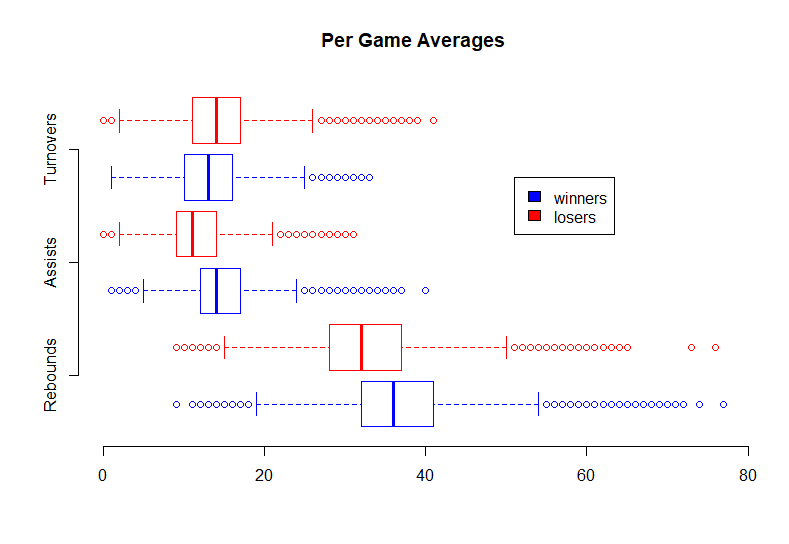
\includegraphics[scale=0.255]{GameAverages.png}
		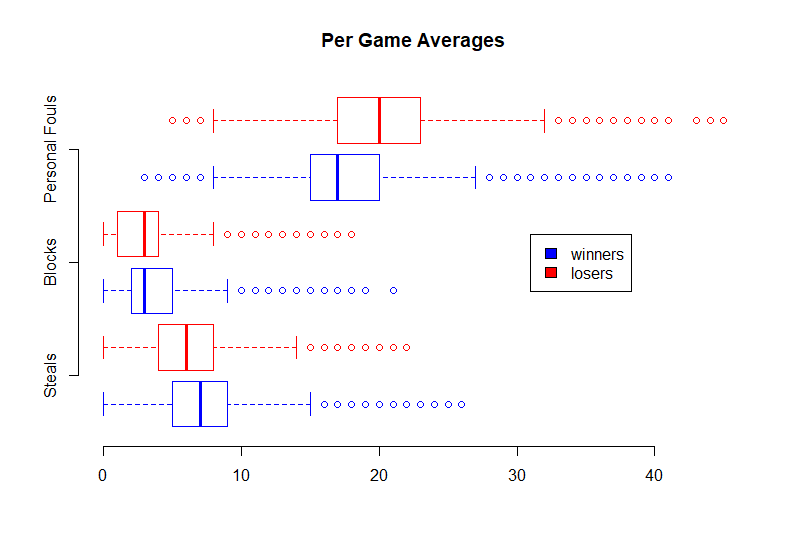
\includegraphics[scale=0.255]{GameAverages2.png}  
	\end{center}
\footnotesize \center  Winning teams hold higher averages in "positive" stats such as assists, rebounds, and steals. 
\frametitle{{\textbf{\huge Pre-Analysis}}}
\end{frame}
\begin{frame}
\begin{center}
	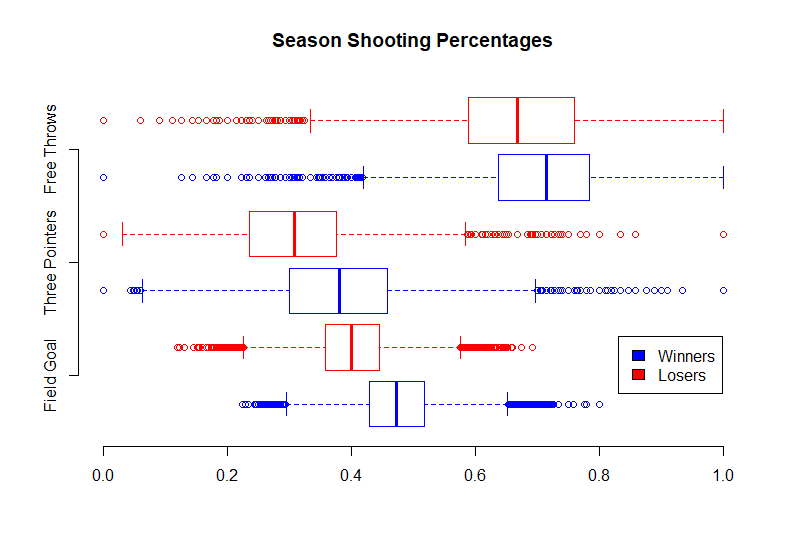
\includegraphics[scale=0.255]{SeasonShotPercent.png}
	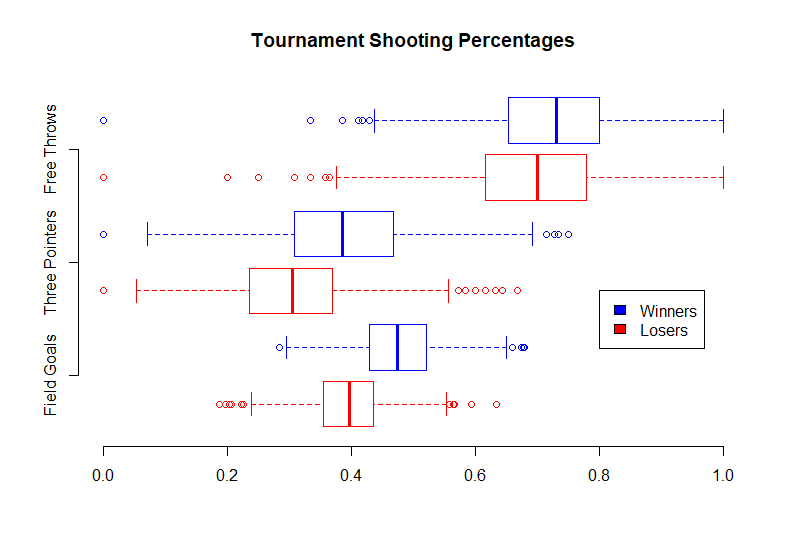
\includegraphics[scale=0.255]{TourneyShotPercent.png}  
\end{center}
\footnotesize \center As anticipated, the winning teams averaged higher in all categories, but there are a significant number of outliers in the Season data.
\frametitle{{\textbf{\huge Pre-Analysis}}}
\end{frame}
\begin{frame}
\begin{center}
	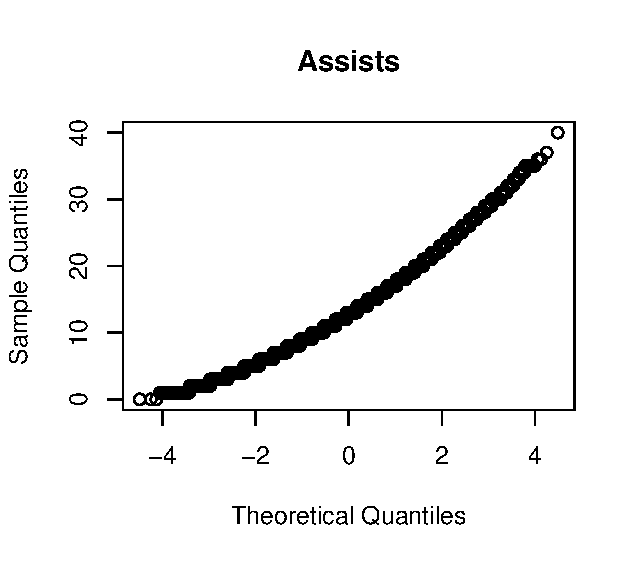
\includegraphics[scale=0.33]{assnorm.pdf}
	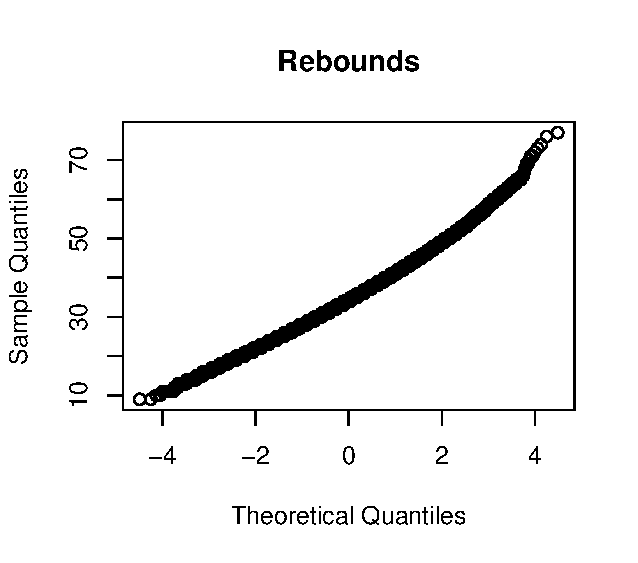
\includegraphics[scale=0.33]{rbnorm.pdf}
	\includegraphics[scale=0.33]{FGnorm.pdf} 
\end{center}
\footnotesize\center We examined the distribution of parameters of interset. Unsurpisnigly , due to the large sample size, the variables are normally distributed.
\frametitle{{\textbf{\huge Pre-Analysis}}}
\end{frame}
\begin{frame}
\begin{figure}[H]
	\centering
	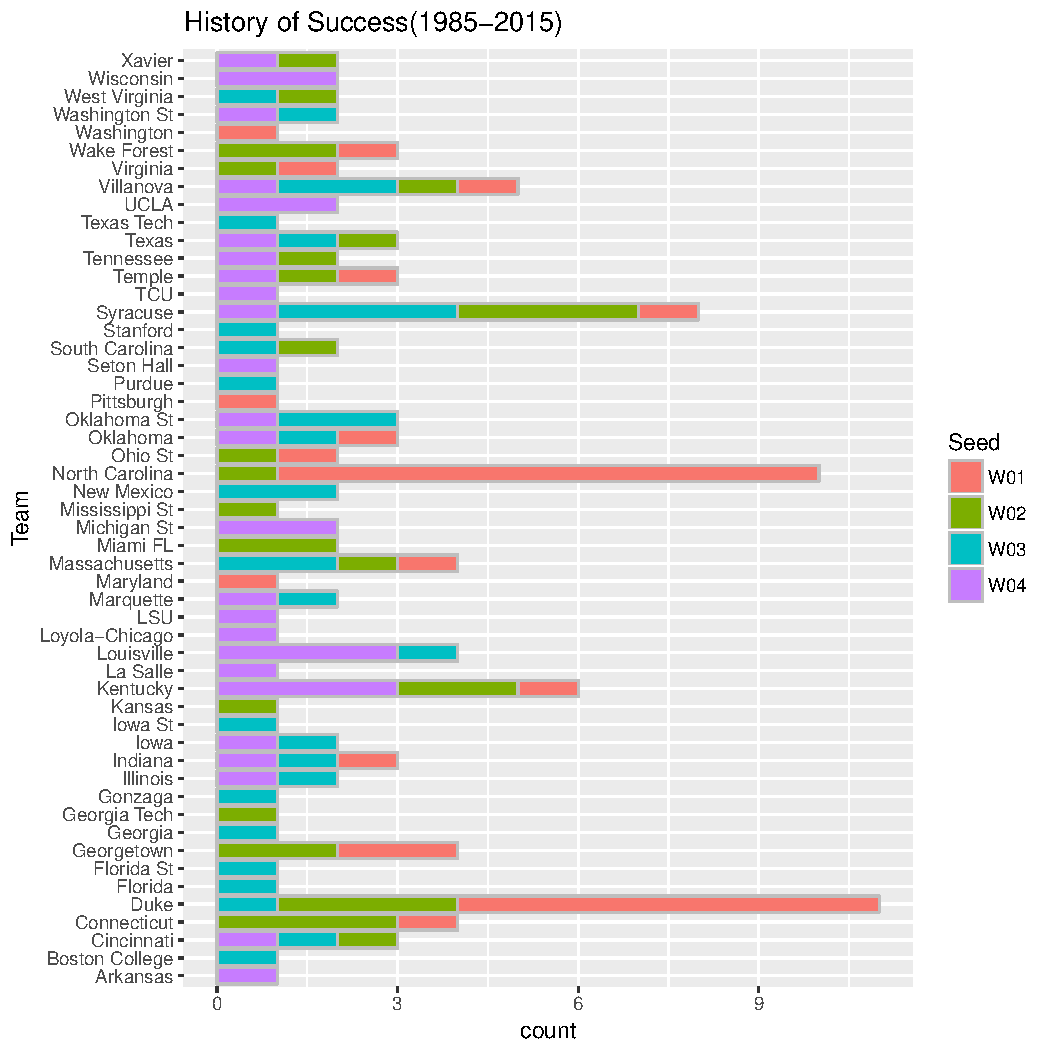
\includegraphics[scale=.35]{HistOfSuccess.pdf}
\end{figure}
\frametitle{{\textbf{\huge Pre-Analysis}}}
\end{frame}
\section{Initial Model}
\begin{frame}
	\[
	Y_{daynum} = \beta_0 + \beta_{conf} + \beta_{fgp} +\beta_{tpp} + \beta_{ass} + \beta_{rb} + \beta_{app} + \epsilon
	\]
	\footnotesize We initially looked into this model, where the betas represented the following:
\begin{itemize}
	\item conf: the conference the team plays in
	\item fgp: the field goal percentages
	\item tpp: three point shooting percentage
	\item ass: assists
	\item rb: rebounds
	\item app: prior tournament success
\end{itemize}
\frametitle{{\textbf{\huge Initial Model}}}
\end{frame}
\section{Process}
\begin{frame}
In processing our data to develop the model, we went through a number of steps:
\begin{itemize}
	\footnotesize
	\item Separate out the needed data for each team for each year
	\item Eliminate unusable predictors, and search out missing values
	\item Calculate the averages of each team's stats for each year
	\item Compile the averages into a new csv file that we could use moving forward
	\item Develop a process for representing how far a team has made it in the tournament
\end{itemize}
\frametitle{{\textbf{\huge Processing}}}
\end{frame}
\begin{frame}
\center We quantified our response variable by keeping record of how many games each team plays in the tournament each year, where better teams would be expected to play more games. This did leave us with a lot of missing values(all the teams who didn't make the tournament), so we experimented with models to find how to handle this.
\frametitle{{\textbf{\huge Processing}}}
\end{frame}
\section{Final Model}
\begin{frame}
We looked into quite a few models before settling on a single one to work with. We analyzed the models for each year and found some variation from year to year caused by:
\footnotesize
\begin{itemize}
	\item Upsets in the tournament
	\item Great stats in the season but no slot in the tournament (can depend on conference)
\end{itemize}
\frametitle{{\textbf{\huge Final Model}}}
\end{frame}
\section{Model Analysis}
\begin{frame}
\frametitle{{\textbf{\huge Model Analysis}}}
\end{frame}
\begin{frame}
\begin{center}
	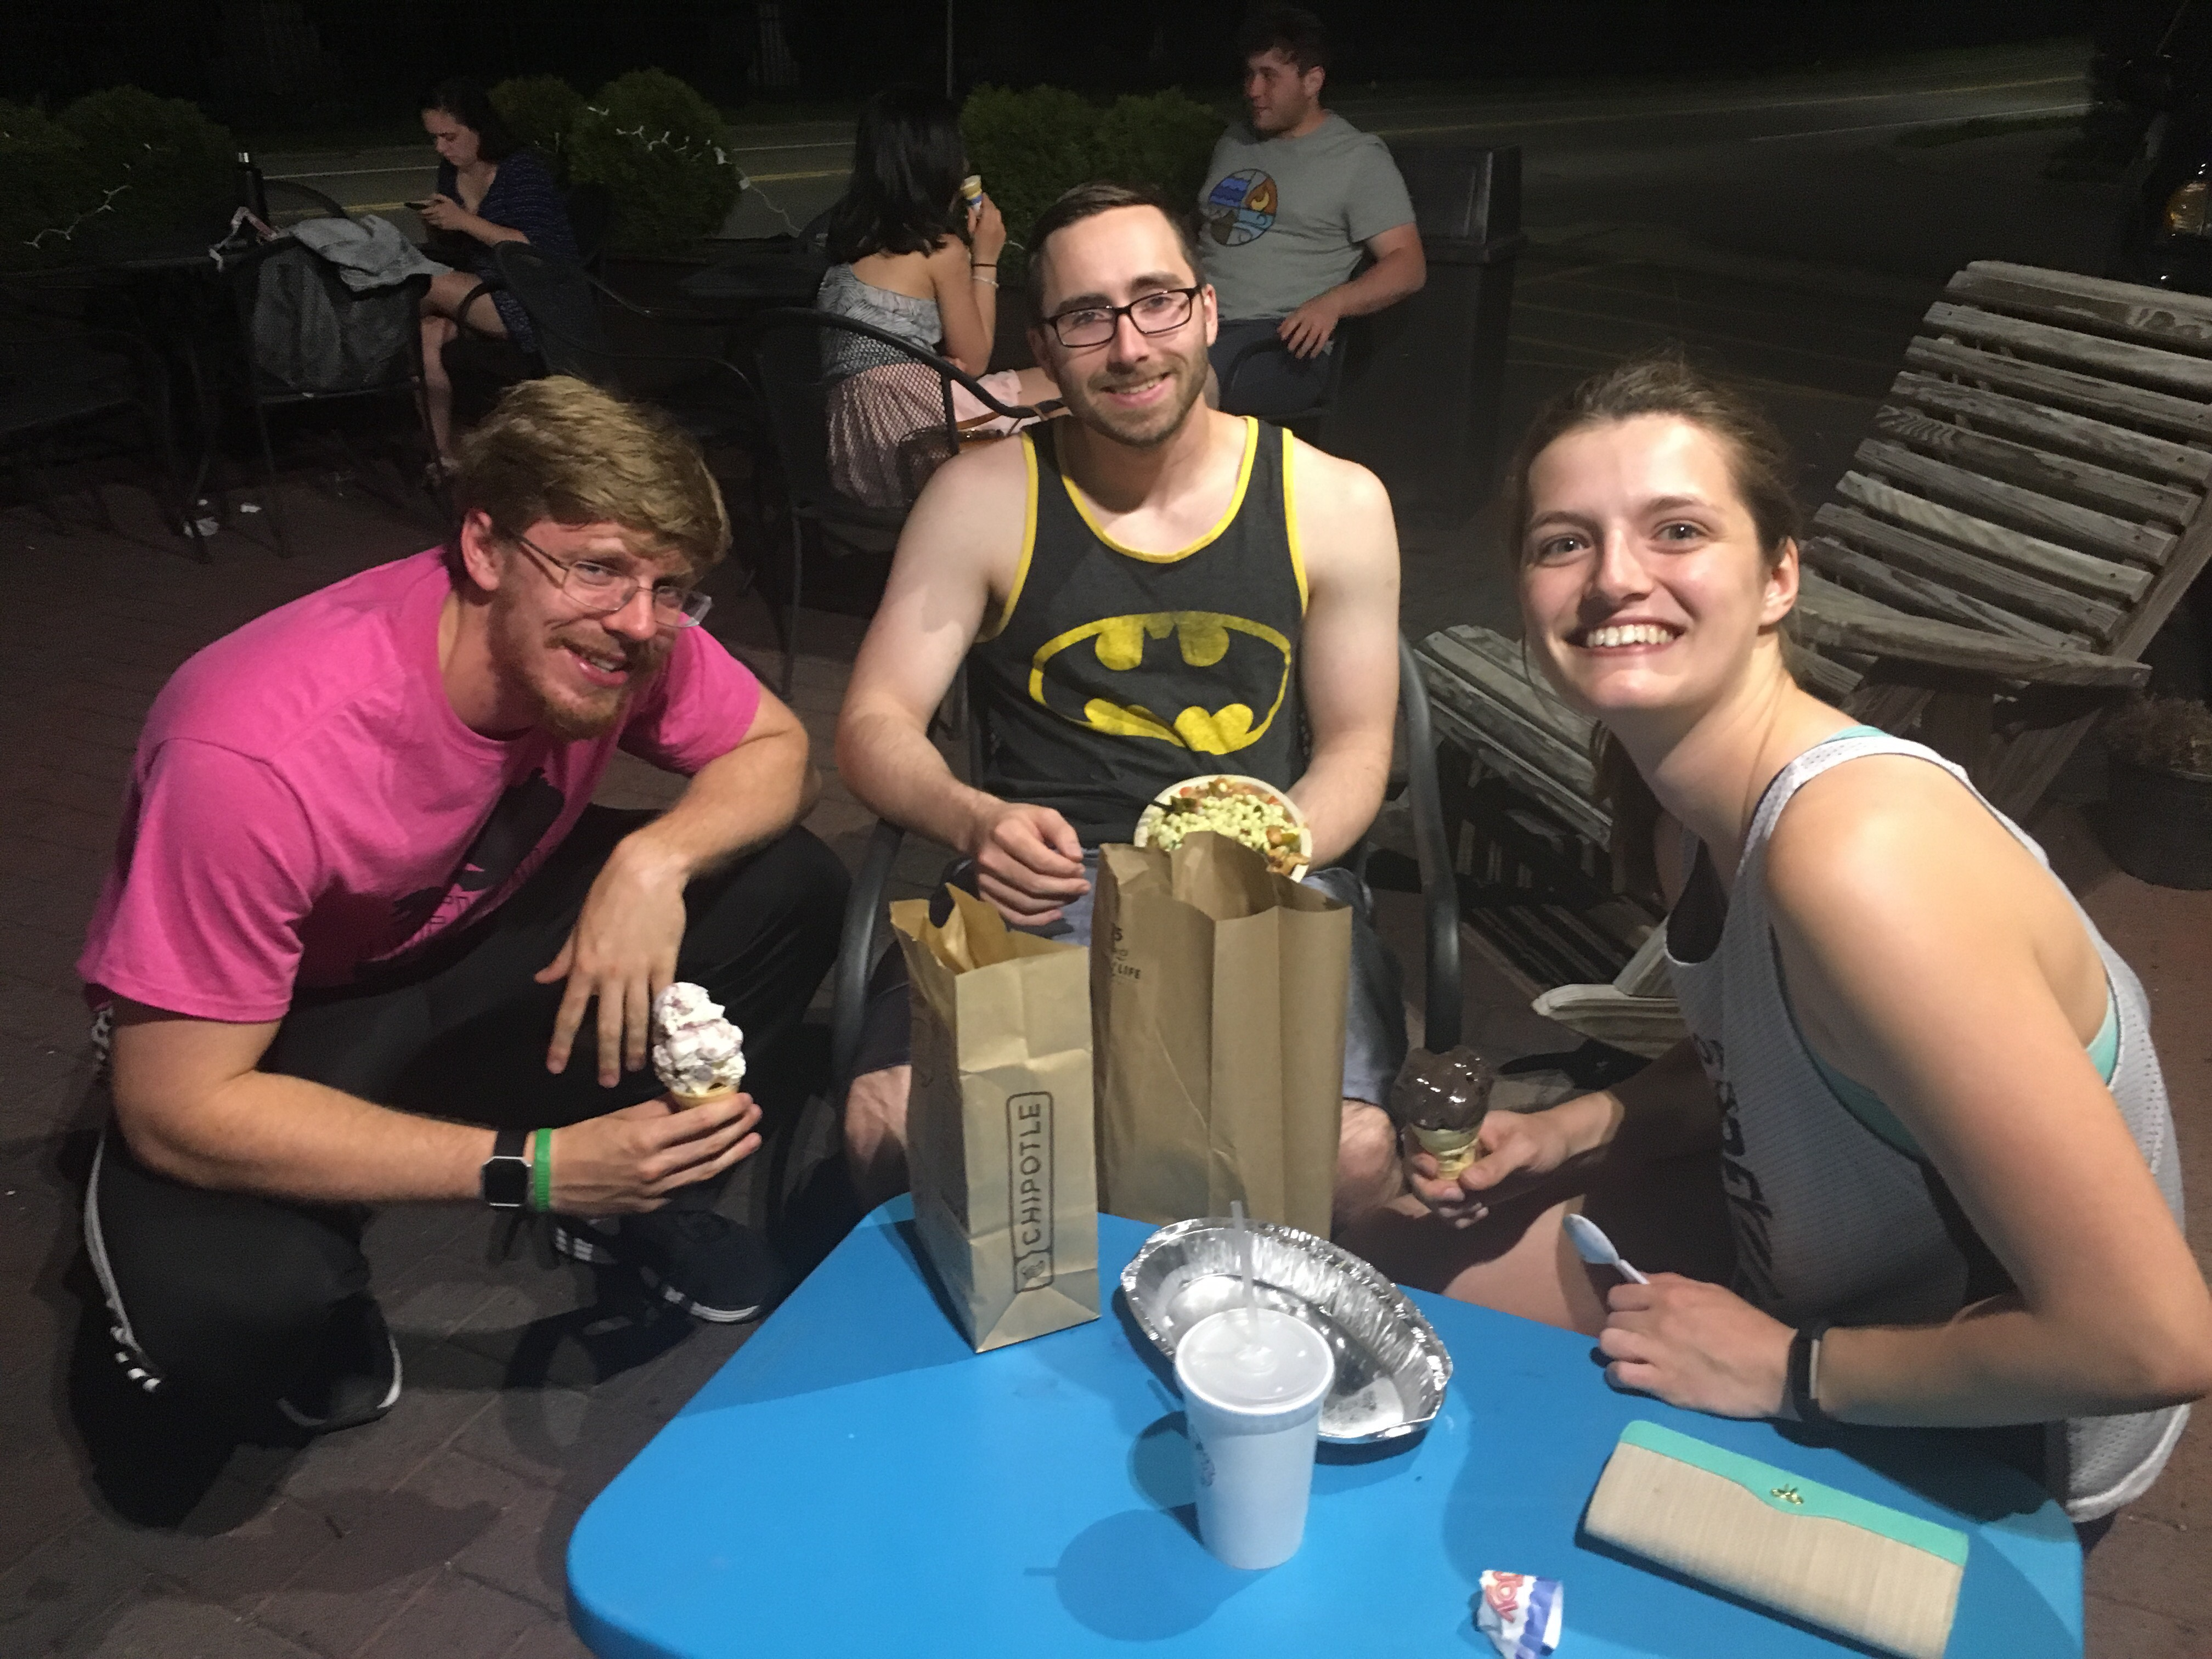
\includegraphics[scale=0.05]{questions.jpg} 
\end{center}
\frametitle{{\textbf{\huge Questions?}}}
\end{frame}

\end{document}